% Created by tikzDevice version 0.12.6 on 2026-09-09 19:44:34
% !TEX encoding = UTF-8 Unicode
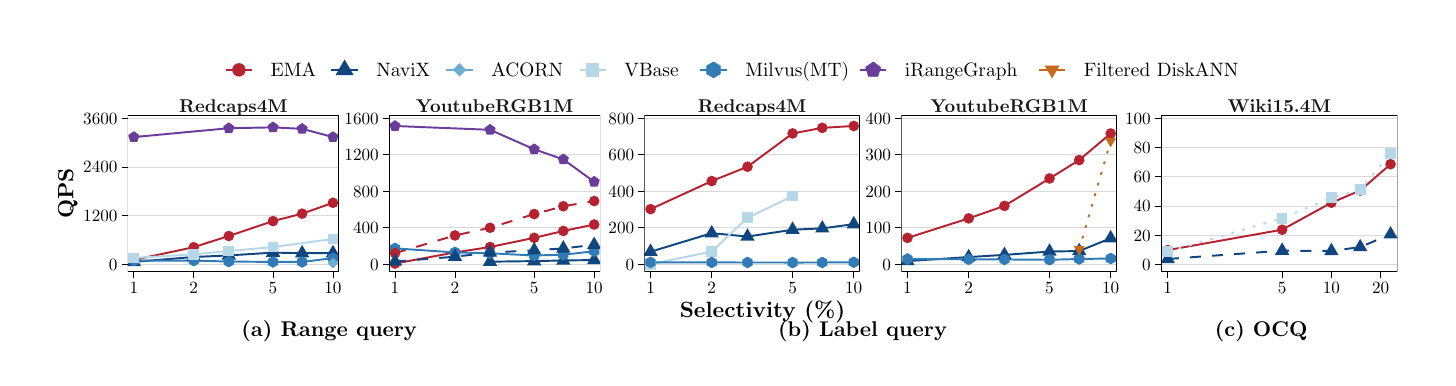
\begin{tikzpicture}[x=1pt,y=1pt]
\definecolor{fillColor}{RGB}{255,255,255}
\path[use as bounding box,fill=fillColor,fill opacity=0.00] (0,0) rectangle (505.89,119.25);
\begin{scope}
\path[clip] (  0.00,  0.00) rectangle (505.89,119.25);
\definecolor{drawColor}{RGB}{255,255,255}
\definecolor{fillColor}{RGB}{255,255,255}

\path[draw=drawColor,line width= 0.6pt,line join=round,line cap=round,fill=fillColor] (  0.00,  0.00) rectangle (505.89,119.25);
\end{scope}
\begin{scope}
\path[clip] (  5.50, 94.27) rectangle (500.39,113.75);
\definecolor{drawColor}{RGB}{255,255,255}
\definecolor{fillColor}{RGB}{255,255,255}

\path[draw=drawColor,line width= 0.6pt,line join=round,line cap=round,fill=fillColor] (  5.50, 94.27) rectangle (500.39,113.75);
\end{scope}
\begin{scope}
\path[clip] (  0.00,  0.00) rectangle (505.89,119.25);
\definecolor{drawColor}{RGB}{183,34,48}

\path[draw=drawColor,line width= 0.7pt,line join=round] ( 71.56,104.01) -- ( 81.12,104.01);
\definecolor{fillColor}{RGB}{183,34,48}

\path[fill=fillColor] ( 76.34,104.01) circle (  2.43);
\end{scope}
\begin{scope}
\path[clip] (  0.00,  0.00) rectangle (505.89,119.25);
\definecolor{drawColor}{RGB}{16,70,128}

\path[draw=drawColor,line width= 0.7pt,line join=round] (109.74,104.01) -- (119.30,104.01);
\definecolor{fillColor}{RGB}{16,70,128}

\path[fill=fillColor] (114.52,107.78) --
	(117.79,102.12) --
	(111.25,102.12) --
	cycle;
\end{scope}
\begin{scope}
\path[clip] (  0.00,  0.00) rectangle (505.89,119.25);
\definecolor{drawColor}{RGB}{109,173,209}

\path[draw=drawColor,line width= 0.7pt,line join=round] (151.29,104.01) -- (160.85,104.01);
\definecolor{fillColor}{RGB}{109,173,209}

\path[fill=fillColor] (153.64,104.01) --
	(156.07,106.44) --
	(158.50,104.01) --
	(156.07,101.58) --
	cycle;
\end{scope}
\begin{scope}
\path[clip] (  0.00,  0.00) rectangle (505.89,119.25);
\definecolor{drawColor}{RGB}{182,215,232}

\path[draw=drawColor,line width= 0.7pt,line join=round] (199.40,104.01) -- (208.96,104.01);
\definecolor{fillColor}{RGB}{182,215,232}

\path[fill=fillColor] (201.75,101.58) --
	(206.61,101.58) --
	(206.61,106.44) --
	(201.75,106.44) --
	cycle;
\end{scope}
\begin{scope}
\path[clip] (  0.00,  0.00) rectangle (505.89,119.25);
\definecolor{drawColor}{RGB}{49,124,183}

\path[draw=drawColor,line width= 0.7pt,line join=round] (243.05,104.01) -- (252.61,104.01);
\definecolor{fillColor}{RGB}{49,124,183}

\path[draw=drawColor,line width= 0.2pt,line join=round,line cap=round,fill=fillColor] (250.32,105.45) --
	(247.83,106.89) --
	(245.34,105.45) --
	(245.34,102.57) --
	(247.83,101.13) --
	(250.32,102.57) --
	(250.32,105.45) --
	cycle;
\end{scope}
\begin{scope}
\path[clip] (  0.00,  0.00) rectangle (505.89,119.25);
\definecolor{drawColor}{RGB}{106,61,154}

\path[draw=drawColor,line width= 0.7pt,line join=round] (300.73,104.01) -- (310.29,104.01);
\definecolor{fillColor}{RGB}{106,61,154}

\path[draw=drawColor,line width= 0.2pt,line join=round,line cap=round,fill=fillColor] (305.51,106.89) --
	(302.77,104.90) --
	(303.82,101.68) --
	(307.20,101.68) --
	(308.25,104.90) --
	(305.51,106.89) --
	cycle;
\end{scope}
\begin{scope}
\path[clip] (  0.00,  0.00) rectangle (505.89,119.25);
\definecolor{drawColor}{RGB}{198,106,27}

\path[draw=drawColor,line width= 0.7pt,line join=round] (365.40,104.01) -- (374.96,104.01);
\definecolor{fillColor}{RGB}{198,106,27}

\path[draw=drawColor,line width= 0.2pt,line join=round,line cap=round,fill=fillColor] (370.18,101.13) --
	(372.67,105.45) --
	(367.68,105.45) --
	(370.18,101.13) --
	cycle;
\end{scope}
\begin{scope}
\path[clip] (  0.00,  0.00) rectangle (505.89,119.25);
\definecolor{drawColor}{RGB}{0,0,0}

\node[text=drawColor,anchor=base west,inner sep=0pt, outer sep=0pt, scale=  0.70] at ( 87.82,101.60) {EMA};
\end{scope}
\begin{scope}
\path[clip] (  0.00,  0.00) rectangle (505.89,119.25);
\definecolor{drawColor}{RGB}{0,0,0}

\node[text=drawColor,anchor=base west,inner sep=0pt, outer sep=0pt, scale=  0.70] at (126.00,101.60) {NaviX};
\end{scope}
\begin{scope}
\path[clip] (  0.00,  0.00) rectangle (505.89,119.25);
\definecolor{drawColor}{RGB}{0,0,0}

\node[text=drawColor,anchor=base west,inner sep=0pt, outer sep=0pt, scale=  0.70] at (167.54,101.60) {ACORN};
\end{scope}
\begin{scope}
\path[clip] (  0.00,  0.00) rectangle (505.89,119.25);
\definecolor{drawColor}{RGB}{0,0,0}

\node[text=drawColor,anchor=base west,inner sep=0pt, outer sep=0pt, scale=  0.70] at (215.66,101.60) {VBase};
\end{scope}
\begin{scope}
\path[clip] (  0.00,  0.00) rectangle (505.89,119.25);
\definecolor{drawColor}{RGB}{0,0,0}

\node[text=drawColor,anchor=base west,inner sep=0pt, outer sep=0pt, scale=  0.70] at (259.30,101.60) {Milvus(MT)};
\end{scope}
\begin{scope}
\path[clip] (  0.00,  0.00) rectangle (505.89,119.25);
\definecolor{drawColor}{RGB}{0,0,0}

\node[text=drawColor,anchor=base west,inner sep=0pt, outer sep=0pt, scale=  0.70] at (316.99,101.60) {iRangeGraph};
\end{scope}
\begin{scope}
\path[clip] (  0.00,  0.00) rectangle (505.89,119.25);
\definecolor{drawColor}{RGB}{0,0,0}

\node[text=drawColor,anchor=base west,inner sep=0pt, outer sep=0pt, scale=  0.70] at (381.65,101.60) {Filtered DiskANN};
\end{scope}
\begin{scope}
\path[clip] (  5.50,  5.50) rectangle (208.36, 94.27);
\definecolor{fillColor}{RGB}{255,255,255}

\path[fill=fillColor] (  5.50,  5.50) rectangle (208.36, 94.27);
\end{scope}
\begin{scope}
\path[clip] (208.36,  5.50) rectangle (395.04, 94.27);
\definecolor{fillColor}{RGB}{255,255,255}

\path[fill=fillColor] (208.36,  5.50) rectangle (395.04, 94.27);
\end{scope}
\begin{scope}
\path[clip] (395.04,  5.50) rectangle (500.39, 94.27);
\definecolor{fillColor}{RGB}{255,255,255}

\path[fill=fillColor] (395.04,  5.50) rectangle (500.39, 94.27);
\end{scope}
\begin{scope}
\path[clip] ( 36.19, 31.08) rectangle (112.47, 87.55);
\definecolor{fillColor}{RGB}{255,255,255}

\path[fill=fillColor] ( 36.19, 31.08) rectangle (112.47, 87.55);
\definecolor{drawColor}{gray}{0.85}

\path[draw=drawColor,line width= 0.3pt,line join=round] ( 36.19, 33.72) --
	(112.47, 33.72);

\path[draw=drawColor,line width= 0.3pt,line join=round] ( 36.19, 51.31) --
	(112.47, 51.31);

\path[draw=drawColor,line width= 0.3pt,line join=round] ( 36.19, 68.90) --
	(112.47, 68.90);

\path[draw=drawColor,line width= 0.3pt,line join=round] ( 36.19, 86.49) --
	(112.47, 86.49);
\definecolor{drawColor}{RGB}{183,34,48}

\path[draw=drawColor,line width= 0.7pt,line join=round] ( 38.35, 35.32) --
	( 60.01, 39.93) --
	( 72.68, 43.97) --
	( 88.65, 49.36) --
	( 99.17, 52.04) --
	(110.31, 55.97);
\definecolor{drawColor}{RGB}{106,61,154}

\path[draw=drawColor,line width= 0.7pt,line join=round] ( 38.35, 79.71) --
	( 72.68, 82.92) --
	( 88.65, 83.22) --
	( 99.17, 82.69) --
	(110.31, 79.72);
\definecolor{drawColor}{RGB}{16,70,128}

\path[draw=drawColor,line width= 0.7pt,line join=round] ( 38.35, 34.63) --
	( 60.01, 36.38) --
	( 72.68, 36.95) --
	( 88.65, 37.97) --
	( 99.17, 37.76) --
	(110.31, 37.79);
\definecolor{drawColor}{RGB}{182,215,232}

\path[draw=drawColor,line width= 0.7pt,line join=round] ( 38.35, 36.05) --
	( 60.01, 37.34) --
	( 72.68, 38.56) --
	( 88.65, 39.98) --
	(110.31, 42.88);
\definecolor{drawColor}{RGB}{49,124,183}

\path[draw=drawColor,line width= 0.7pt,line join=round] ( 38.35, 35.10) --
	( 60.01, 35.09) --
	( 72.68, 34.74) --
	( 88.65, 34.60) --
	( 99.17, 34.59) --
	(110.31, 35.96);
\definecolor{fillColor}{RGB}{183,34,48}

\path[fill=fillColor] (110.31, 55.97) circle (  1.93);

\path[fill=fillColor] ( 99.17, 52.04) circle (  1.93);

\path[fill=fillColor] ( 88.65, 49.36) circle (  1.93);

\path[fill=fillColor] ( 72.68, 43.97) circle (  1.93);

\path[fill=fillColor] ( 60.01, 39.93) circle (  1.93);

\path[fill=fillColor] ( 38.35, 35.32) circle (  1.93);
\definecolor{drawColor}{RGB}{106,61,154}
\definecolor{fillColor}{RGB}{106,61,154}

\path[draw=drawColor,line width= 0.5pt,line join=round,line cap=round,fill=fillColor] (110.31, 81.55) --
	(108.56, 80.28) --
	(109.23, 78.23) --
	(111.39, 78.23) --
	(112.06, 80.28) --
	(110.31, 81.55) --
	cycle;
\end{scope}
\begin{scope}
\path[clip] ( 36.19, 31.08) rectangle (112.47, 87.55);
\definecolor{drawColor}{RGB}{106,61,154}
\definecolor{fillColor}{RGB}{106,61,154}

\path[draw=drawColor,line width= 0.5pt,line join=round,line cap=round,fill=fillColor] ( 99.17, 84.53) --
	( 97.42, 83.26) --
	( 98.08, 81.21) --
	(100.25, 81.21) --
	(100.91, 83.26) --
	( 99.17, 84.53) --
	cycle;
\end{scope}
\begin{scope}
\path[clip] ( 36.19, 31.08) rectangle (112.47, 87.55);
\definecolor{drawColor}{RGB}{106,61,154}
\definecolor{fillColor}{RGB}{106,61,154}

\path[draw=drawColor,line width= 0.5pt,line join=round,line cap=round,fill=fillColor] ( 88.65, 85.06) --
	( 86.90, 83.79) --
	( 87.57, 81.73) --
	( 89.73, 81.73) --
	( 90.40, 83.79) --
	( 88.65, 85.06) --
	cycle;
\end{scope}
\begin{scope}
\path[clip] ( 36.19, 31.08) rectangle (112.47, 87.55);
\definecolor{drawColor}{RGB}{106,61,154}
\definecolor{fillColor}{RGB}{106,61,154}

\path[draw=drawColor,line width= 0.5pt,line join=round,line cap=round,fill=fillColor] ( 72.68, 84.75) --
	( 70.94, 83.48) --
	( 71.60, 81.43) --
	( 73.76, 81.43) --
	( 74.43, 83.48) --
	( 72.68, 84.75) --
	cycle;
\end{scope}
\begin{scope}
\path[clip] ( 36.19, 31.08) rectangle (112.47, 87.55);
\definecolor{drawColor}{RGB}{106,61,154}
\definecolor{fillColor}{RGB}{106,61,154}

\path[draw=drawColor,line width= 0.5pt,line join=round,line cap=round,fill=fillColor] ( 38.35, 81.55) --
	( 36.60, 80.28) --
	( 37.27, 78.23) --
	( 39.43, 78.23) --
	( 40.10, 80.28) --
	( 38.35, 81.55) --
	cycle;
\end{scope}
\begin{scope}
\path[clip] ( 36.19, 31.08) rectangle (112.47, 87.55);
\definecolor{fillColor}{RGB}{16,70,128}

\path[fill=fillColor] (110.31, 40.79) --
	(112.91, 36.29) --
	(107.72, 36.29) --
	cycle;

\path[fill=fillColor] ( 99.17, 40.76) --
	(101.76, 36.27) --
	( 96.57, 36.27) --
	cycle;

\path[fill=fillColor] ( 88.65, 40.97) --
	( 91.25, 36.47) --
	( 86.05, 36.47) --
	cycle;

\path[fill=fillColor] ( 72.68, 39.95) --
	( 75.28, 35.45) --
	( 70.09, 35.45) --
	cycle;

\path[fill=fillColor] ( 60.01, 39.38) --
	( 62.61, 34.89) --
	( 57.42, 34.89) --
	cycle;

\path[fill=fillColor] ( 38.35, 37.63) --
	( 40.94, 33.13) --
	( 35.75, 33.13) --
	cycle;
\definecolor{drawColor}{RGB}{49,124,183}
\definecolor{fillColor}{RGB}{49,124,183}

\path[draw=drawColor,line width= 0.5pt,line join=round,line cap=round,fill=fillColor] (111.90, 36.88) --
	(110.31, 37.80) --
	(108.72, 36.88) --
	(108.72, 35.04) --
	(110.31, 34.12) --
	(111.90, 35.04) --
	(111.90, 36.88) --
	cycle;
\end{scope}
\begin{scope}
\path[clip] ( 36.19, 31.08) rectangle (112.47, 87.55);
\definecolor{drawColor}{RGB}{49,124,183}
\definecolor{fillColor}{RGB}{49,124,183}

\path[draw=drawColor,line width= 0.5pt,line join=round,line cap=round,fill=fillColor] (100.76, 35.51) --
	( 99.17, 36.42) --
	( 97.57, 35.51) --
	( 97.57, 33.67) --
	( 99.17, 32.75) --
	(100.76, 33.67) --
	(100.76, 35.51) --
	cycle;
\end{scope}
\begin{scope}
\path[clip] ( 36.19, 31.08) rectangle (112.47, 87.55);
\definecolor{drawColor}{RGB}{49,124,183}
\definecolor{fillColor}{RGB}{49,124,183}

\path[draw=drawColor,line width= 0.5pt,line join=round,line cap=round,fill=fillColor] ( 90.24, 35.52) --
	( 88.65, 36.43) --
	( 87.06, 35.52) --
	( 87.06, 33.68) --
	( 88.65, 32.76) --
	( 90.24, 33.68) --
	( 90.24, 35.52) --
	cycle;
\end{scope}
\begin{scope}
\path[clip] ( 36.19, 31.08) rectangle (112.47, 87.55);
\definecolor{drawColor}{RGB}{49,124,183}
\definecolor{fillColor}{RGB}{49,124,183}

\path[draw=drawColor,line width= 0.5pt,line join=round,line cap=round,fill=fillColor] ( 74.28, 35.66) --
	( 72.68, 36.58) --
	( 71.09, 35.66) --
	( 71.09, 33.82) --
	( 72.68, 32.90) --
	( 74.28, 33.82) --
	( 74.28, 35.66) --
	cycle;
\end{scope}
\begin{scope}
\path[clip] ( 36.19, 31.08) rectangle (112.47, 87.55);
\definecolor{drawColor}{RGB}{49,124,183}
\definecolor{fillColor}{RGB}{49,124,183}

\path[draw=drawColor,line width= 0.5pt,line join=round,line cap=round,fill=fillColor] ( 61.60, 36.01) --
	( 60.01, 36.93) --
	( 58.42, 36.01) --
	( 58.42, 34.17) --
	( 60.01, 33.25) --
	( 61.60, 34.17) --
	( 61.60, 36.01) --
	cycle;
\end{scope}
\begin{scope}
\path[clip] ( 36.19, 31.08) rectangle (112.47, 87.55);
\definecolor{drawColor}{RGB}{49,124,183}
\definecolor{fillColor}{RGB}{49,124,183}

\path[draw=drawColor,line width= 0.5pt,line join=round,line cap=round,fill=fillColor] ( 39.94, 36.01) --
	( 38.35, 36.93) --
	( 36.76, 36.01) --
	( 36.76, 34.18) --
	( 38.35, 33.26) --
	( 39.94, 34.18) --
	( 39.94, 36.01) --
	cycle;
\end{scope}
\begin{scope}
\path[clip] ( 36.19, 31.08) rectangle (112.47, 87.55);
\definecolor{fillColor}{RGB}{109,173,209}

\path[fill=fillColor] (108.38, 34.16) --
	(110.31, 36.08) --
	(112.24, 34.16) --
	(110.31, 32.23) --
	cycle;
\definecolor{fillColor}{RGB}{182,215,232}

\path[fill=fillColor] (108.38, 40.95) --
	(112.24, 40.95) --
	(112.24, 44.81) --
	(108.38, 44.81) --
	cycle;

\path[fill=fillColor] ( 86.72, 38.05) --
	( 90.58, 38.05) --
	( 90.58, 41.90) --
	( 86.72, 41.90) --
	cycle;

\path[fill=fillColor] ( 70.76, 36.63) --
	( 74.61, 36.63) --
	( 74.61, 40.49) --
	( 70.76, 40.49) --
	cycle;

\path[fill=fillColor] ( 58.08, 35.41) --
	( 61.94, 35.41) --
	( 61.94, 39.26) --
	( 58.08, 39.26) --
	cycle;

\path[fill=fillColor] ( 36.42, 34.13) --
	( 40.28, 34.13) --
	( 40.28, 37.98) --
	( 36.42, 37.98) --
	cycle;
\definecolor{drawColor}{RGB}{0,0,0}

\path[draw=drawColor,line width= 0.4pt,line join=round,line cap=round] ( 36.19, 31.08) rectangle (112.47, 87.55);
\end{scope}
\begin{scope}
\path[clip] (130.58, 31.08) rectangle (206.86, 87.55);
\definecolor{fillColor}{RGB}{255,255,255}

\path[fill=fillColor] (130.58, 31.08) rectangle (206.86, 87.55);
\definecolor{drawColor}{gray}{0.85}

\path[draw=drawColor,line width= 0.3pt,line join=round] (130.58, 33.72) --
	(206.86, 33.72);

\path[draw=drawColor,line width= 0.3pt,line join=round] (130.58, 46.91) --
	(206.86, 46.91);

\path[draw=drawColor,line width= 0.3pt,line join=round] (130.58, 60.11) --
	(206.86, 60.11);

\path[draw=drawColor,line width= 0.3pt,line join=round] (130.58, 73.30) --
	(206.86, 73.30);

\path[draw=drawColor,line width= 0.3pt,line join=round] (130.58, 86.49) --
	(206.86, 86.49);
\definecolor{drawColor}{RGB}{183,34,48}

\path[draw=drawColor,line width= 0.7pt,line join=round] (132.74, 34.01) --
	(154.40, 38.04) --
	(167.07, 39.99) --
	(183.04, 43.31) --
	(193.55, 45.79) --
	(204.70, 48.12);

\path[draw=drawColor,line width= 0.7pt,dash pattern=on 4pt off 4pt ,line join=round] (132.74, 37.76) --
	(154.40, 44.17) --
	(167.07, 46.94) --
	(183.04, 51.90) --
	(193.55, 54.71) --
	(204.70, 56.60);
\definecolor{drawColor}{RGB}{106,61,154}

\path[draw=drawColor,line width= 0.7pt,line join=round] (132.74, 83.72) --
	(167.07, 82.34) --
	(183.04, 75.31) --
	(193.55, 71.65) --
	(204.70, 63.57);
\definecolor{drawColor}{RGB}{16,70,128}

\path[draw=drawColor,line width= 0.7pt,line join=round] (167.07, 34.69) --
	(183.04, 34.90) --
	(193.55, 35.13) --
	(204.70, 35.28);

\path[draw=drawColor,line width= 0.7pt,dash pattern=on 4pt off 4pt ,line join=round] (132.74, 34.74) --
	(154.40, 36.50) --
	(167.07, 37.97) --
	(183.04, 38.82) --
	(193.55, 39.48) --
	(204.70, 40.78);
\definecolor{drawColor}{RGB}{49,124,183}

\path[draw=drawColor,line width= 0.7pt,line join=round] (132.74, 39.50) --
	(154.40, 38.04) --
	(167.07, 37.72) --
	(183.04, 36.94) --
	(193.55, 37.19) --
	(204.70, 38.47);
\definecolor{fillColor}{RGB}{183,34,48}

\path[fill=fillColor] (204.70, 48.12) circle (  1.93);

\path[fill=fillColor] (193.55, 45.79) circle (  1.93);

\path[fill=fillColor] (183.04, 43.31) circle (  1.93);

\path[fill=fillColor] (167.07, 39.99) circle (  1.93);

\path[fill=fillColor] (154.40, 38.04) circle (  1.93);

\path[fill=fillColor] (132.74, 34.01) circle (  1.93);
\definecolor{drawColor}{RGB}{106,61,154}
\definecolor{fillColor}{RGB}{106,61,154}

\path[draw=drawColor,line width= 0.5pt,line join=round,line cap=round,fill=fillColor] (204.70, 65.41) --
	(202.95, 64.14) --
	(203.62, 62.08) --
	(205.78, 62.08) --
	(206.45, 64.14) --
	(204.70, 65.41) --
	cycle;
\end{scope}
\begin{scope}
\path[clip] (130.58, 31.08) rectangle (206.86, 87.55);
\definecolor{drawColor}{RGB}{106,61,154}
\definecolor{fillColor}{RGB}{106,61,154}

\path[draw=drawColor,line width= 0.5pt,line join=round,line cap=round,fill=fillColor] (193.55, 73.49) --
	(191.80, 72.22) --
	(192.47, 70.16) --
	(194.63, 70.16) --
	(195.30, 72.22) --
	(193.55, 73.49) --
	cycle;
\end{scope}
\begin{scope}
\path[clip] (130.58, 31.08) rectangle (206.86, 87.55);
\definecolor{drawColor}{RGB}{106,61,154}
\definecolor{fillColor}{RGB}{106,61,154}

\path[draw=drawColor,line width= 0.5pt,line join=round,line cap=round,fill=fillColor] (183.04, 77.15) --
	(181.29, 75.88) --
	(181.96, 73.82) --
	(184.12, 73.82) --
	(184.78, 75.88) --
	(183.04, 77.15) --
	cycle;
\end{scope}
\begin{scope}
\path[clip] (130.58, 31.08) rectangle (206.86, 87.55);
\definecolor{drawColor}{RGB}{106,61,154}
\definecolor{fillColor}{RGB}{106,61,154}

\path[draw=drawColor,line width= 0.5pt,line join=round,line cap=round,fill=fillColor] (167.07, 84.17) --
	(165.32, 82.90) --
	(165.99, 80.85) --
	(168.15, 80.85) --
	(168.82, 82.90) --
	(167.07, 84.17) --
	cycle;
\end{scope}
\begin{scope}
\path[clip] (130.58, 31.08) rectangle (206.86, 87.55);
\definecolor{drawColor}{RGB}{106,61,154}
\definecolor{fillColor}{RGB}{106,61,154}

\path[draw=drawColor,line width= 0.5pt,line join=round,line cap=round,fill=fillColor] (132.74, 85.56) --
	(130.99, 84.29) --
	(131.65, 82.24) --
	(133.82, 82.24) --
	(134.48, 84.29) --
	(132.74, 85.56) --
	cycle;
\end{scope}
\begin{scope}
\path[clip] (130.58, 31.08) rectangle (206.86, 87.55);
\definecolor{fillColor}{RGB}{16,70,128}

\path[fill=fillColor] (204.70, 38.28) --
	(207.30, 33.78) --
	(202.10, 33.78) --
	cycle;

\path[fill=fillColor] (193.55, 38.13) --
	(196.15, 33.63) --
	(190.96, 33.63) --
	cycle;

\path[fill=fillColor] (183.04, 37.90) --
	(185.63, 33.40) --
	(180.44, 33.40) --
	cycle;

\path[fill=fillColor] (167.07, 37.69) --
	(169.67, 33.19) --
	(164.47, 33.19) --
	cycle;
\definecolor{drawColor}{RGB}{49,124,183}
\definecolor{fillColor}{RGB}{49,124,183}

\path[draw=drawColor,line width= 0.5pt,line join=round,line cap=round,fill=fillColor] (206.29, 39.39) --
	(204.70, 40.31) --
	(203.11, 39.39) --
	(203.11, 37.55) --
	(204.70, 36.63) --
	(206.29, 37.55) --
	(206.29, 39.39) --
	cycle;
\end{scope}
\begin{scope}
\path[clip] (130.58, 31.08) rectangle (206.86, 87.55);
\definecolor{drawColor}{RGB}{49,124,183}
\definecolor{fillColor}{RGB}{49,124,183}

\path[draw=drawColor,line width= 0.5pt,line join=round,line cap=round,fill=fillColor] (195.14, 38.11) --
	(193.55, 39.03) --
	(191.96, 38.11) --
	(191.96, 36.27) --
	(193.55, 35.35) --
	(195.14, 36.27) --
	(195.14, 38.11) --
	cycle;
\end{scope}
\begin{scope}
\path[clip] (130.58, 31.08) rectangle (206.86, 87.55);
\definecolor{drawColor}{RGB}{49,124,183}
\definecolor{fillColor}{RGB}{49,124,183}

\path[draw=drawColor,line width= 0.5pt,line join=round,line cap=round,fill=fillColor] (184.63, 37.85) --
	(183.04, 38.77) --
	(181.44, 37.85) --
	(181.44, 36.02) --
	(183.04, 35.10) --
	(184.63, 36.02) --
	(184.63, 37.85) --
	cycle;
\end{scope}
\begin{scope}
\path[clip] (130.58, 31.08) rectangle (206.86, 87.55);
\definecolor{drawColor}{RGB}{49,124,183}
\definecolor{fillColor}{RGB}{49,124,183}

\path[draw=drawColor,line width= 0.5pt,line join=round,line cap=round,fill=fillColor] (168.66, 38.64) --
	(167.07, 39.55) --
	(165.48, 38.64) --
	(165.48, 36.80) --
	(167.07, 35.88) --
	(168.66, 36.80) --
	(168.66, 38.64) --
	cycle;
\end{scope}
\begin{scope}
\path[clip] (130.58, 31.08) rectangle (206.86, 87.55);
\definecolor{drawColor}{RGB}{49,124,183}
\definecolor{fillColor}{RGB}{49,124,183}

\path[draw=drawColor,line width= 0.5pt,line join=round,line cap=round,fill=fillColor] (155.99, 38.96) --
	(154.40, 39.87) --
	(152.81, 38.96) --
	(152.81, 37.12) --
	(154.40, 36.20) --
	(155.99, 37.12) --
	(155.99, 38.96) --
	cycle;
\end{scope}
\begin{scope}
\path[clip] (130.58, 31.08) rectangle (206.86, 87.55);
\definecolor{drawColor}{RGB}{49,124,183}
\definecolor{fillColor}{RGB}{49,124,183}

\path[draw=drawColor,line width= 0.5pt,line join=round,line cap=round,fill=fillColor] (134.33, 40.41) --
	(132.74, 41.33) --
	(131.14, 40.41) --
	(131.14, 38.58) --
	(132.74, 37.66) --
	(134.33, 38.58) --
	(134.33, 40.41) --
	cycle;
\end{scope}
\begin{scope}
\path[clip] (130.58, 31.08) rectangle (206.86, 87.55);
\definecolor{fillColor}{RGB}{183,34,48}

\path[fill=fillColor] (204.70, 56.60) circle (  1.93);

\path[fill=fillColor] (193.55, 54.71) circle (  1.93);

\path[fill=fillColor] (183.04, 51.90) circle (  1.93);

\path[fill=fillColor] (167.07, 46.94) circle (  1.93);

\path[fill=fillColor] (154.40, 44.17) circle (  1.93);

\path[fill=fillColor] (132.74, 37.76) circle (  1.93);
\definecolor{fillColor}{RGB}{16,70,128}

\path[fill=fillColor] (204.70, 43.78) --
	(207.30, 39.28) --
	(202.10, 39.28) --
	cycle;

\path[fill=fillColor] (193.55, 42.48) --
	(196.15, 37.98) --
	(190.96, 37.98) --
	cycle;

\path[fill=fillColor] (183.04, 41.81) --
	(185.63, 37.32) --
	(180.44, 37.32) --
	cycle;

\path[fill=fillColor] (167.07, 40.97) --
	(169.67, 36.48) --
	(164.47, 36.48) --
	cycle;

\path[fill=fillColor] (154.40, 39.50) --
	(156.99, 35.00) --
	(151.80, 35.00) --
	cycle;

\path[fill=fillColor] (132.74, 37.74) --
	(135.33, 33.24) --
	(130.14, 33.24) --
	cycle;
\definecolor{drawColor}{RGB}{0,0,0}

\path[draw=drawColor,line width= 0.4pt,line join=round,line cap=round] (130.58, 31.08) rectangle (206.86, 87.55);
\end{scope}
\begin{scope}
\path[clip] (  0.00,  0.00) rectangle (505.89,119.25);
\definecolor{drawColor}{RGB}{0,0,0}

\node[text=drawColor,anchor=base east,inner sep=0pt, outer sep=0pt, scale=  0.62] at (126.86, 31.58) {0};

\node[text=drawColor,anchor=base east,inner sep=0pt, outer sep=0pt, scale=  0.62] at (126.86, 44.78) {400};

\node[text=drawColor,anchor=base east,inner sep=0pt, outer sep=0pt, scale=  0.62] at (126.86, 57.97) {800};

\node[text=drawColor,anchor=base east,inner sep=0pt, outer sep=0pt, scale=  0.62] at (126.86, 71.16) {1200};

\node[text=drawColor,anchor=base east,inner sep=0pt, outer sep=0pt, scale=  0.62] at (126.86, 84.36) {1600};
\end{scope}
\begin{scope}
\path[clip] (  0.00,  0.00) rectangle (505.89,119.25);
\definecolor{drawColor}{RGB}{0,0,0}

\path[draw=drawColor,line width= 0.3pt,line join=round] (128.30, 33.72) --
	(130.58, 33.72);

\path[draw=drawColor,line width= 0.3pt,line join=round] (128.30, 46.91) --
	(130.58, 46.91);

\path[draw=drawColor,line width= 0.3pt,line join=round] (128.30, 60.11) --
	(130.58, 60.11);

\path[draw=drawColor,line width= 0.3pt,line join=round] (128.30, 73.30) --
	(130.58, 73.30);

\path[draw=drawColor,line width= 0.3pt,line join=round] (128.30, 86.49) --
	(130.58, 86.49);
\end{scope}
\begin{scope}
\path[clip] ( 36.19, 87.55) rectangle (112.47, 93.77);
\definecolor{fillColor}{RGB}{255,255,255}

\path[fill=fillColor] ( 36.19, 87.55) rectangle (112.47, 93.77);
\definecolor{drawColor}{gray}{0.10}

\node[text=drawColor,anchor=base,inner sep=0pt, outer sep=0pt, scale=  0.67] at ( 74.33, 88.50) {\bfseries Redcaps4M};
\end{scope}
\begin{scope}
\path[clip] (130.58, 87.55) rectangle (206.86, 93.77);
\definecolor{fillColor}{RGB}{255,255,255}

\path[fill=fillColor] (130.58, 87.55) rectangle (206.86, 93.77);
\definecolor{drawColor}{gray}{0.10}

\node[text=drawColor,anchor=base,inner sep=0pt, outer sep=0pt, scale=  0.67] at (168.72, 88.50) {\bfseries YoutubeRGB1M};
\end{scope}
\begin{scope}
\path[clip] (  0.00,  0.00) rectangle (505.89,119.25);
\definecolor{drawColor}{RGB}{0,0,0}

\path[draw=drawColor,line width= 0.3pt,line join=round] ( 38.35, 28.80) --
	( 38.35, 31.08);

\path[draw=drawColor,line width= 0.3pt,line join=round] ( 60.01, 28.80) --
	( 60.01, 31.08);

\path[draw=drawColor,line width= 0.3pt,line join=round] ( 88.65, 28.80) --
	( 88.65, 31.08);

\path[draw=drawColor,line width= 0.3pt,line join=round] (110.31, 28.80) --
	(110.31, 31.08);
\end{scope}
\begin{scope}
\path[clip] (  0.00,  0.00) rectangle (505.89,119.25);
\definecolor{drawColor}{RGB}{0,0,0}

\node[text=drawColor,anchor=base,inner sep=0pt, outer sep=0pt, scale=  0.62] at ( 38.35, 23.09) {1};

\node[text=drawColor,anchor=base,inner sep=0pt, outer sep=0pt, scale=  0.62] at ( 60.01, 23.09) {2};

\node[text=drawColor,anchor=base,inner sep=0pt, outer sep=0pt, scale=  0.62] at ( 88.65, 23.09) {5};

\node[text=drawColor,anchor=base,inner sep=0pt, outer sep=0pt, scale=  0.62] at (110.31, 23.09) {10};
\end{scope}
\begin{scope}
\path[clip] (  0.00,  0.00) rectangle (505.89,119.25);
\definecolor{drawColor}{RGB}{0,0,0}

\path[draw=drawColor,line width= 0.3pt,line join=round] (132.74, 28.80) --
	(132.74, 31.08);

\path[draw=drawColor,line width= 0.3pt,line join=round] (154.40, 28.80) --
	(154.40, 31.08);

\path[draw=drawColor,line width= 0.3pt,line join=round] (183.04, 28.80) --
	(183.04, 31.08);

\path[draw=drawColor,line width= 0.3pt,line join=round] (204.70, 28.80) --
	(204.70, 31.08);
\end{scope}
\begin{scope}
\path[clip] (  0.00,  0.00) rectangle (505.89,119.25);
\definecolor{drawColor}{RGB}{0,0,0}

\node[text=drawColor,anchor=base,inner sep=0pt, outer sep=0pt, scale=  0.62] at (132.74, 23.09) {1};

\node[text=drawColor,anchor=base,inner sep=0pt, outer sep=0pt, scale=  0.62] at (154.40, 23.09) {2};

\node[text=drawColor,anchor=base,inner sep=0pt, outer sep=0pt, scale=  0.62] at (183.04, 23.09) {5};

\node[text=drawColor,anchor=base,inner sep=0pt, outer sep=0pt, scale=  0.62] at (204.70, 23.09) {10};
\end{scope}
\begin{scope}
\path[clip] (  0.00,  0.00) rectangle (505.89,119.25);
\definecolor{drawColor}{RGB}{0,0,0}

\node[text=drawColor,anchor=base east,inner sep=0pt, outer sep=0pt, scale=  0.62] at ( 32.47, 31.58) {0};

\node[text=drawColor,anchor=base east,inner sep=0pt, outer sep=0pt, scale=  0.62] at ( 32.47, 49.17) {1200};

\node[text=drawColor,anchor=base east,inner sep=0pt, outer sep=0pt, scale=  0.62] at ( 32.47, 66.77) {2400};

\node[text=drawColor,anchor=base east,inner sep=0pt, outer sep=0pt, scale=  0.62] at ( 32.47, 84.36) {3600};
\end{scope}
\begin{scope}
\path[clip] (  0.00,  0.00) rectangle (505.89,119.25);
\definecolor{drawColor}{RGB}{0,0,0}

\path[draw=drawColor,line width= 0.3pt,line join=round] ( 33.91, 33.72) --
	( 36.19, 33.72);

\path[draw=drawColor,line width= 0.3pt,line join=round] ( 33.91, 51.31) --
	( 36.19, 51.31);

\path[draw=drawColor,line width= 0.3pt,line join=round] ( 33.91, 68.90) --
	( 36.19, 68.90);

\path[draw=drawColor,line width= 0.3pt,line join=round] ( 33.91, 86.49) --
	( 36.19, 86.49);
\end{scope}
\begin{scope}
\path[clip] (  0.00,  0.00) rectangle (505.89,119.25);
\definecolor{drawColor}{RGB}{0,0,0}

\node[text=drawColor,rotate= 90.00,anchor=base,inner sep=0pt, outer sep=0pt, scale=  0.80] at ( 16.52, 59.31) {\bfseries QPS};
\end{scope}
\begin{scope}
\path[clip] (  0.00,  0.00) rectangle (505.89,119.25);
\definecolor{drawColor}{RGB}{0,0,0}

\node[text=drawColor,anchor=base,inner sep=0pt, outer sep=0pt, scale=  0.77] at (108.93,  7.50) {\bfseries (a) Range query};
\end{scope}
\begin{scope}
\path[clip] (222.87, 31.08) rectangle (300.70, 87.55);
\definecolor{fillColor}{RGB}{255,255,255}

\path[fill=fillColor] (222.87, 31.08) rectangle (300.70, 87.55);
\definecolor{drawColor}{gray}{0.85}

\path[draw=drawColor,line width= 0.3pt,line join=round] (222.87, 33.72) --
	(300.70, 33.72);

\path[draw=drawColor,line width= 0.3pt,line join=round] (222.87, 46.91) --
	(300.70, 46.91);

\path[draw=drawColor,line width= 0.3pt,line join=round] (222.87, 60.11) --
	(300.70, 60.11);

\path[draw=drawColor,line width= 0.3pt,line join=round] (222.87, 73.30) --
	(300.70, 73.30);

\path[draw=drawColor,line width= 0.3pt,line join=round] (222.87, 86.49) --
	(300.70, 86.49);
\definecolor{drawColor}{RGB}{183,34,48}

\path[draw=drawColor,line width= 0.7pt,line join=round] (225.08, 53.67) --
	(247.18, 63.82) --
	(260.11, 69.00) --
	(276.40, 81.03) --
	(287.13, 83.05) --
	(298.50, 83.73);
\definecolor{drawColor}{RGB}{16,70,128}

\path[draw=drawColor,line width= 0.7pt,line join=round] (225.08, 38.29) --
	(247.18, 44.99) --
	(260.11, 43.77) --
	(276.40, 46.24) --
	(287.13, 46.73) --
	(298.50, 48.25);
\definecolor{drawColor}{RGB}{182,215,232}

\path[draw=drawColor,line width= 0.7pt,line join=round] (225.08, 33.77) --
	(247.18, 38.36) --
	(260.11, 50.56) --
	(276.40, 58.39);
\definecolor{drawColor}{RGB}{49,124,183}

\path[draw=drawColor,line width= 0.7pt,line join=round] (225.08, 34.45) --
	(247.18, 34.42) --
	(260.11, 34.40) --
	(276.40, 34.38) --
	(287.13, 34.39) --
	(298.50, 34.48);
\definecolor{fillColor}{RGB}{183,34,48}

\path[fill=fillColor] (298.50, 83.73) circle (  1.93);

\path[fill=fillColor] (287.13, 83.05) circle (  1.93);

\path[fill=fillColor] (276.40, 81.03) circle (  1.93);

\path[fill=fillColor] (260.11, 69.00) circle (  1.93);

\path[fill=fillColor] (247.18, 63.82) circle (  1.93);

\path[fill=fillColor] (225.08, 53.67) circle (  1.93);
\definecolor{fillColor}{RGB}{16,70,128}

\path[fill=fillColor] (298.50, 51.25) --
	(301.10, 46.75) --
	(295.91, 46.75) --
	cycle;

\path[fill=fillColor] (287.13, 49.73) --
	(289.72, 45.24) --
	(284.53, 45.24) --
	cycle;

\path[fill=fillColor] (276.40, 49.24) --
	(278.99, 44.74) --
	(273.80, 44.74) --
	cycle;

\path[fill=fillColor] (260.11, 46.76) --
	(262.70, 42.27) --
	(257.51, 42.27) --
	cycle;

\path[fill=fillColor] (247.18, 47.98) --
	(249.77, 43.49) --
	(244.58, 43.49) --
	cycle;

\path[fill=fillColor] (225.08, 41.28) --
	(227.67, 36.79) --
	(222.48, 36.79) --
	cycle;
\definecolor{fillColor}{RGB}{182,215,232}

\path[fill=fillColor] (274.47, 56.46) --
	(278.33, 56.46) --
	(278.33, 60.32) --
	(274.47, 60.32) --
	cycle;

\path[fill=fillColor] (258.18, 48.63) --
	(262.04, 48.63) --
	(262.04, 52.49) --
	(258.18, 52.49) --
	cycle;

\path[fill=fillColor] (245.25, 36.43) --
	(249.11, 36.43) --
	(249.11, 40.28) --
	(245.25, 40.28) --
	cycle;

\path[fill=fillColor] (223.15, 31.84) --
	(227.00, 31.84) --
	(227.00, 35.69) --
	(223.15, 35.69) --
	cycle;
\definecolor{fillColor}{RGB}{49,124,183}

\path[draw=drawColor,line width= 0.5pt,line join=round,line cap=round,fill=fillColor] (300.09, 35.40) --
	(298.50, 36.31) --
	(296.91, 35.40) --
	(296.91, 33.56) --
	(298.50, 32.64) --
	(300.09, 33.56) --
	(300.09, 35.40) --
	cycle;
\end{scope}
\begin{scope}
\path[clip] (222.87, 31.08) rectangle (300.70, 87.55);
\definecolor{drawColor}{RGB}{49,124,183}
\definecolor{fillColor}{RGB}{49,124,183}

\path[draw=drawColor,line width= 0.5pt,line join=round,line cap=round,fill=fillColor] (288.72, 35.31) --
	(287.13, 36.23) --
	(285.54, 35.31) --
	(285.54, 33.48) --
	(287.13, 32.56) --
	(288.72, 33.48) --
	(288.72, 35.31) --
	cycle;
\end{scope}
\begin{scope}
\path[clip] (222.87, 31.08) rectangle (300.70, 87.55);
\definecolor{drawColor}{RGB}{49,124,183}
\definecolor{fillColor}{RGB}{49,124,183}

\path[draw=drawColor,line width= 0.5pt,line join=round,line cap=round,fill=fillColor] (277.99, 35.30) --
	(276.40, 36.22) --
	(274.81, 35.30) --
	(274.81, 33.46) --
	(276.40, 32.54) --
	(277.99, 33.46) --
	(277.99, 35.30) --
	cycle;
\end{scope}
\begin{scope}
\path[clip] (222.87, 31.08) rectangle (300.70, 87.55);
\definecolor{drawColor}{RGB}{49,124,183}
\definecolor{fillColor}{RGB}{49,124,183}

\path[draw=drawColor,line width= 0.5pt,line join=round,line cap=round,fill=fillColor] (261.70, 35.32) --
	(260.11, 36.24) --
	(258.52, 35.32) --
	(258.52, 33.49) --
	(260.11, 32.57) --
	(261.70, 33.49) --
	(261.70, 35.32) --
	cycle;
\end{scope}
\begin{scope}
\path[clip] (222.87, 31.08) rectangle (300.70, 87.55);
\definecolor{drawColor}{RGB}{49,124,183}
\definecolor{fillColor}{RGB}{49,124,183}

\path[draw=drawColor,line width= 0.5pt,line join=round,line cap=round,fill=fillColor] (248.77, 35.34) --
	(247.18, 36.26) --
	(245.59, 35.34) --
	(245.59, 33.50) --
	(247.18, 32.58) --
	(248.77, 33.50) --
	(248.77, 35.34) --
	cycle;
\end{scope}
\begin{scope}
\path[clip] (222.87, 31.08) rectangle (300.70, 87.55);
\definecolor{drawColor}{RGB}{49,124,183}
\definecolor{fillColor}{RGB}{49,124,183}

\path[draw=drawColor,line width= 0.5pt,line join=round,line cap=round,fill=fillColor] (226.67, 35.37) --
	(225.08, 36.29) --
	(223.48, 35.37) --
	(223.48, 33.53) --
	(225.08, 32.61) --
	(226.67, 33.53) --
	(226.67, 35.37) --
	cycle;
\end{scope}
\begin{scope}
\path[clip] (222.87, 31.08) rectangle (300.70, 87.55);
\definecolor{drawColor}{RGB}{0,0,0}

\path[draw=drawColor,line width= 0.4pt,line join=round,line cap=round] (222.87, 31.08) rectangle (300.70, 87.55);
\end{scope}
\begin{scope}
\path[clip] (315.71, 31.08) rectangle (393.54, 87.55);
\definecolor{fillColor}{RGB}{255,255,255}

\path[fill=fillColor] (315.71, 31.08) rectangle (393.54, 87.55);
\definecolor{drawColor}{gray}{0.85}

\path[draw=drawColor,line width= 0.3pt,line join=round] (315.71, 33.72) --
	(393.54, 33.72);

\path[draw=drawColor,line width= 0.3pt,line join=round] (315.71, 46.91) --
	(393.54, 46.91);

\path[draw=drawColor,line width= 0.3pt,line join=round] (315.71, 60.11) --
	(393.54, 60.11);

\path[draw=drawColor,line width= 0.3pt,line join=round] (315.71, 73.30) --
	(393.54, 73.30);

\path[draw=drawColor,line width= 0.3pt,line join=round] (315.71, 86.49) --
	(393.54, 86.49);
\definecolor{drawColor}{RGB}{183,34,48}

\path[draw=drawColor,line width= 0.7pt,line join=round] (317.91, 43.29) --
	(340.02, 50.33) --
	(352.95, 54.85) --
	(369.24, 64.75) --
	(379.96, 71.40) --
	(391.34, 81.02);
\definecolor{drawColor}{RGB}{16,70,128}

\path[draw=drawColor,line width= 0.7pt,line join=round] (317.91, 34.91) --
	(340.02, 36.36) --
	(352.95, 37.15) --
	(369.24, 38.35) --
	(379.96, 38.54) --
	(391.34, 43.16);
\definecolor{drawColor}{RGB}{49,124,183}

\path[draw=drawColor,line width= 0.7pt,line join=round] (317.91, 35.67) --
	(340.02, 35.54) --
	(352.95, 35.49) --
	(369.24, 35.38) --
	(379.96, 35.66) --
	(391.34, 35.83);
\definecolor{drawColor}{RGB}{198,106,27}

\path[draw=drawColor,line width= 0.7pt,dash pattern=on 1pt off 3pt ,line join=round] (379.96, 39.23) --
	(391.34, 78.28);
\definecolor{fillColor}{RGB}{183,34,48}

\path[fill=fillColor] (391.34, 81.02) circle (  1.93);

\path[fill=fillColor] (379.96, 71.40) circle (  1.93);

\path[fill=fillColor] (369.24, 64.75) circle (  1.93);

\path[fill=fillColor] (352.95, 54.85) circle (  1.93);

\path[fill=fillColor] (340.02, 50.33) circle (  1.93);

\path[fill=fillColor] (317.91, 43.29) circle (  1.93);
\definecolor{fillColor}{RGB}{16,70,128}

\path[fill=fillColor] (391.34, 46.16) --
	(393.93, 41.66) --
	(388.74, 41.66) --
	cycle;

\path[fill=fillColor] (379.96, 41.54) --
	(382.56, 37.04) --
	(377.37, 37.04) --
	cycle;

\path[fill=fillColor] (369.24, 41.35) --
	(371.83, 36.85) --
	(366.64, 36.85) --
	cycle;

\path[fill=fillColor] (352.95, 40.15) --
	(355.54, 35.65) --
	(350.35, 35.65) --
	cycle;

\path[fill=fillColor] (340.02, 39.36) --
	(342.61, 34.86) --
	(337.42, 34.86) --
	cycle;

\path[fill=fillColor] (317.91, 37.91) --
	(320.51, 33.41) --
	(315.32, 33.41) --
	cycle;
\definecolor{drawColor}{RGB}{49,124,183}
\definecolor{fillColor}{RGB}{49,124,183}

\path[draw=drawColor,line width= 0.5pt,line join=round,line cap=round,fill=fillColor] (392.93, 36.75) --
	(391.34, 37.67) --
	(389.75, 36.75) --
	(389.75, 34.91) --
	(391.34, 34.00) --
	(392.93, 34.91) --
	(392.93, 36.75) --
	cycle;
\end{scope}
\begin{scope}
\path[clip] (315.71, 31.08) rectangle (393.54, 87.55);
\definecolor{drawColor}{RGB}{49,124,183}
\definecolor{fillColor}{RGB}{49,124,183}

\path[draw=drawColor,line width= 0.5pt,line join=round,line cap=round,fill=fillColor] (381.56, 36.58) --
	(379.96, 37.49) --
	(378.37, 36.58) --
	(378.37, 34.74) --
	(379.96, 33.82) --
	(381.56, 34.74) --
	(381.56, 36.58) --
	cycle;
\end{scope}
\begin{scope}
\path[clip] (315.71, 31.08) rectangle (393.54, 87.55);
\definecolor{drawColor}{RGB}{49,124,183}
\definecolor{fillColor}{RGB}{49,124,183}

\path[draw=drawColor,line width= 0.5pt,line join=round,line cap=round,fill=fillColor] (370.83, 36.30) --
	(369.24, 37.22) --
	(367.64, 36.30) --
	(367.64, 34.46) --
	(369.24, 33.54) --
	(370.83, 34.46) --
	(370.83, 36.30) --
	cycle;
\end{scope}
\begin{scope}
\path[clip] (315.71, 31.08) rectangle (393.54, 87.55);
\definecolor{drawColor}{RGB}{49,124,183}
\definecolor{fillColor}{RGB}{49,124,183}

\path[draw=drawColor,line width= 0.5pt,line join=round,line cap=round,fill=fillColor] (354.54, 36.41) --
	(352.95, 37.33) --
	(351.35, 36.41) --
	(351.35, 34.57) --
	(352.95, 33.65) --
	(354.54, 34.57) --
	(354.54, 36.41) --
	cycle;
\end{scope}
\begin{scope}
\path[clip] (315.71, 31.08) rectangle (393.54, 87.55);
\definecolor{drawColor}{RGB}{49,124,183}
\definecolor{fillColor}{RGB}{49,124,183}

\path[draw=drawColor,line width= 0.5pt,line join=round,line cap=round,fill=fillColor] (341.61, 36.46) --
	(340.02, 37.38) --
	(338.42, 36.46) --
	(338.42, 34.62) --
	(340.02, 33.70) --
	(341.61, 34.62) --
	(341.61, 36.46) --
	cycle;
\end{scope}
\begin{scope}
\path[clip] (315.71, 31.08) rectangle (393.54, 87.55);
\definecolor{drawColor}{RGB}{49,124,183}
\definecolor{fillColor}{RGB}{49,124,183}

\path[draw=drawColor,line width= 0.5pt,line join=round,line cap=round,fill=fillColor] (319.50, 36.58) --
	(317.91, 37.50) --
	(316.32, 36.58) --
	(316.32, 34.75) --
	(317.91, 33.83) --
	(319.50, 34.75) --
	(319.50, 36.58) --
	cycle;
\end{scope}
\begin{scope}
\path[clip] (315.71, 31.08) rectangle (393.54, 87.55);
\definecolor{drawColor}{RGB}{198,106,27}
\definecolor{fillColor}{RGB}{198,106,27}

\path[draw=drawColor,line width= 0.5pt,line join=round,line cap=round,fill=fillColor] (391.34, 76.44) --
	(392.93, 79.20) --
	(389.75, 79.20) --
	(391.34, 76.44) --
	cycle;
\end{scope}
\begin{scope}
\path[clip] (315.71, 31.08) rectangle (393.54, 87.55);
\definecolor{drawColor}{RGB}{198,106,27}
\definecolor{fillColor}{RGB}{198,106,27}

\path[draw=drawColor,line width= 0.5pt,line join=round,line cap=round,fill=fillColor] (379.96, 37.39) --
	(381.56, 40.15) --
	(378.37, 40.15) --
	(379.96, 37.39) --
	cycle;
\end{scope}
\begin{scope}
\path[clip] (315.71, 31.08) rectangle (393.54, 87.55);
\definecolor{drawColor}{RGB}{0,0,0}

\path[draw=drawColor,line width= 0.4pt,line join=round,line cap=round] (315.71, 31.08) rectangle (393.54, 87.55);
\end{scope}
\begin{scope}
\path[clip] (  0.00,  0.00) rectangle (505.89,119.25);
\definecolor{drawColor}{RGB}{0,0,0}

\node[text=drawColor,anchor=base east,inner sep=0pt, outer sep=0pt, scale=  0.62] at (311.99, 31.58) {0};

\node[text=drawColor,anchor=base east,inner sep=0pt, outer sep=0pt, scale=  0.62] at (311.99, 44.78) {100};

\node[text=drawColor,anchor=base east,inner sep=0pt, outer sep=0pt, scale=  0.62] at (311.99, 57.97) {200};

\node[text=drawColor,anchor=base east,inner sep=0pt, outer sep=0pt, scale=  0.62] at (311.99, 71.16) {300};

\node[text=drawColor,anchor=base east,inner sep=0pt, outer sep=0pt, scale=  0.62] at (311.99, 84.36) {400};
\end{scope}
\begin{scope}
\path[clip] (  0.00,  0.00) rectangle (505.89,119.25);
\definecolor{drawColor}{RGB}{0,0,0}

\path[draw=drawColor,line width= 0.3pt,line join=round] (313.43, 33.72) --
	(315.71, 33.72);

\path[draw=drawColor,line width= 0.3pt,line join=round] (313.43, 46.91) --
	(315.71, 46.91);

\path[draw=drawColor,line width= 0.3pt,line join=round] (313.43, 60.11) --
	(315.71, 60.11);

\path[draw=drawColor,line width= 0.3pt,line join=round] (313.43, 73.30) --
	(315.71, 73.30);

\path[draw=drawColor,line width= 0.3pt,line join=round] (313.43, 86.49) --
	(315.71, 86.49);
\end{scope}
\begin{scope}
\path[clip] (222.87, 87.55) rectangle (300.70, 93.77);
\definecolor{fillColor}{RGB}{255,255,255}

\path[fill=fillColor] (222.87, 87.55) rectangle (300.70, 93.77);
\definecolor{drawColor}{gray}{0.10}

\node[text=drawColor,anchor=base,inner sep=0pt, outer sep=0pt, scale=  0.67] at (261.79, 88.50) {\bfseries Redcaps4M};
\end{scope}
\begin{scope}
\path[clip] (315.71, 87.55) rectangle (393.54, 93.77);
\definecolor{fillColor}{RGB}{255,255,255}

\path[fill=fillColor] (315.71, 87.55) rectangle (393.54, 93.77);
\definecolor{drawColor}{gray}{0.10}

\node[text=drawColor,anchor=base,inner sep=0pt, outer sep=0pt, scale=  0.67] at (354.63, 88.50) {\bfseries YoutubeRGB1M};
\end{scope}
\begin{scope}
\path[clip] (  0.00,  0.00) rectangle (505.89,119.25);
\definecolor{drawColor}{RGB}{0,0,0}

\path[draw=drawColor,line width= 0.3pt,line join=round] (225.08, 28.80) --
	(225.08, 31.08);

\path[draw=drawColor,line width= 0.3pt,line join=round] (247.18, 28.80) --
	(247.18, 31.08);

\path[draw=drawColor,line width= 0.3pt,line join=round] (276.40, 28.80) --
	(276.40, 31.08);

\path[draw=drawColor,line width= 0.3pt,line join=round] (298.50, 28.80) --
	(298.50, 31.08);
\end{scope}
\begin{scope}
\path[clip] (  0.00,  0.00) rectangle (505.89,119.25);
\definecolor{drawColor}{RGB}{0,0,0}

\node[text=drawColor,anchor=base,inner sep=0pt, outer sep=0pt, scale=  0.62] at (225.08, 23.09) {1};

\node[text=drawColor,anchor=base,inner sep=0pt, outer sep=0pt, scale=  0.62] at (247.18, 23.09) {2};

\node[text=drawColor,anchor=base,inner sep=0pt, outer sep=0pt, scale=  0.62] at (276.40, 23.09) {5};

\node[text=drawColor,anchor=base,inner sep=0pt, outer sep=0pt, scale=  0.62] at (298.50, 23.09) {10};
\end{scope}
\begin{scope}
\path[clip] (  0.00,  0.00) rectangle (505.89,119.25);
\definecolor{drawColor}{RGB}{0,0,0}

\path[draw=drawColor,line width= 0.3pt,line join=round] (317.91, 28.80) --
	(317.91, 31.08);

\path[draw=drawColor,line width= 0.3pt,line join=round] (340.02, 28.80) --
	(340.02, 31.08);

\path[draw=drawColor,line width= 0.3pt,line join=round] (369.24, 28.80) --
	(369.24, 31.08);

\path[draw=drawColor,line width= 0.3pt,line join=round] (391.34, 28.80) --
	(391.34, 31.08);
\end{scope}
\begin{scope}
\path[clip] (  0.00,  0.00) rectangle (505.89,119.25);
\definecolor{drawColor}{RGB}{0,0,0}

\node[text=drawColor,anchor=base,inner sep=0pt, outer sep=0pt, scale=  0.62] at (317.91, 23.09) {1};

\node[text=drawColor,anchor=base,inner sep=0pt, outer sep=0pt, scale=  0.62] at (340.02, 23.09) {2};

\node[text=drawColor,anchor=base,inner sep=0pt, outer sep=0pt, scale=  0.62] at (369.24, 23.09) {5};

\node[text=drawColor,anchor=base,inner sep=0pt, outer sep=0pt, scale=  0.62] at (391.34, 23.09) {10};
\end{scope}
\begin{scope}
\path[clip] (  0.00,  0.00) rectangle (505.89,119.25);
\definecolor{drawColor}{RGB}{0,0,0}

\node[text=drawColor,anchor=base east,inner sep=0pt, outer sep=0pt, scale=  0.62] at (219.16, 31.58) {0};

\node[text=drawColor,anchor=base east,inner sep=0pt, outer sep=0pt, scale=  0.62] at (219.16, 44.78) {200};

\node[text=drawColor,anchor=base east,inner sep=0pt, outer sep=0pt, scale=  0.62] at (219.16, 57.97) {400};

\node[text=drawColor,anchor=base east,inner sep=0pt, outer sep=0pt, scale=  0.62] at (219.16, 71.16) {600};

\node[text=drawColor,anchor=base east,inner sep=0pt, outer sep=0pt, scale=  0.62] at (219.16, 84.36) {800};
\end{scope}
\begin{scope}
\path[clip] (  0.00,  0.00) rectangle (505.89,119.25);
\definecolor{drawColor}{RGB}{0,0,0}

\path[draw=drawColor,line width= 0.3pt,line join=round] (220.60, 33.72) --
	(222.87, 33.72);

\path[draw=drawColor,line width= 0.3pt,line join=round] (220.60, 46.91) --
	(222.87, 46.91);

\path[draw=drawColor,line width= 0.3pt,line join=round] (220.60, 60.11) --
	(222.87, 60.11);

\path[draw=drawColor,line width= 0.3pt,line join=round] (220.60, 73.30) --
	(222.87, 73.30);

\path[draw=drawColor,line width= 0.3pt,line join=round] (220.60, 86.49) --
	(222.87, 86.49);
\end{scope}
\begin{scope}
\path[clip] (  0.00,  0.00) rectangle (505.89,119.25);
\definecolor{drawColor}{RGB}{0,0,0}

\node[text=drawColor,anchor=base,inner sep=0pt, outer sep=0pt, scale=  0.77] at (301.70,  7.50) {\bfseries (b) Label query};
\end{scope}
\begin{scope}
\path[clip] (409.56, 31.08) rectangle (494.89, 87.55);
\definecolor{fillColor}{RGB}{255,255,255}

\path[fill=fillColor] (409.56, 31.08) rectangle (494.89, 87.55);
\definecolor{drawColor}{gray}{0.85}

\path[draw=drawColor,line width= 0.3pt,line join=round] (409.56, 33.72) --
	(494.89, 33.72);

\path[draw=drawColor,line width= 0.3pt,line join=round] (409.56, 44.27) --
	(494.89, 44.27);

\path[draw=drawColor,line width= 0.3pt,line join=round] (409.56, 54.83) --
	(494.89, 54.83);

\path[draw=drawColor,line width= 0.3pt,line join=round] (409.56, 65.38) --
	(494.89, 65.38);

\path[draw=drawColor,line width= 0.3pt,line join=round] (409.56, 75.94) --
	(494.89, 75.94);

\path[draw=drawColor,line width= 0.3pt,line join=round] (409.56, 86.49) --
	(494.89, 86.49);
\definecolor{drawColor}{RGB}{183,34,48}

\path[draw=drawColor,line width= 0.7pt,line join=round] (411.97, 38.88) --
	(453.29, 46.25) --
	(471.09, 55.99) --
	(481.50, 60.41) --
	(492.47, 69.91);
\definecolor{drawColor}{RGB}{16,70,128}

\path[draw=drawColor,line width= 0.7pt,dash pattern=on 4pt off 4pt ,line join=round] (411.97, 35.66) --
	(453.29, 38.67) --
	(471.09, 38.55) --
	(481.50, 39.97) --
	(492.47, 44.57);
\definecolor{drawColor}{RGB}{182,215,232}

\path[draw=drawColor,line width= 0.7pt,dash pattern=on 1pt off 3pt ,line join=round] (411.97, 38.29) --
	(453.29, 50.34) --
	(471.09, 57.77) --
	(481.50, 60.65) --
	(492.47, 73.69);
\definecolor{fillColor}{RGB}{183,34,48}

\path[fill=fillColor] (492.47, 69.91) circle (  1.93);

\path[fill=fillColor] (481.50, 60.41) circle (  1.93);

\path[fill=fillColor] (471.09, 55.99) circle (  1.93);

\path[fill=fillColor] (453.29, 46.25) circle (  1.93);

\path[fill=fillColor] (411.97, 38.88) circle (  1.93);
\definecolor{fillColor}{RGB}{16,70,128}

\path[fill=fillColor] (492.47, 47.57) --
	(495.07, 43.07) --
	(489.88, 43.07) --
	cycle;

\path[fill=fillColor] (481.50, 42.96) --
	(484.10, 38.47) --
	(478.90, 38.47) --
	cycle;

\path[fill=fillColor] (471.09, 41.54) --
	(473.69, 37.05) --
	(468.49, 37.05) --
	cycle;

\path[fill=fillColor] (453.29, 41.67) --
	(455.89, 37.17) --
	(450.70, 37.17) --
	cycle;

\path[fill=fillColor] (411.97, 38.66) --
	(414.57, 34.16) --
	(409.37, 34.16) --
	cycle;
\definecolor{fillColor}{RGB}{182,215,232}

\path[fill=fillColor] (490.55, 71.76) --
	(494.40, 71.76) --
	(494.40, 75.62) --
	(490.55, 75.62) --
	cycle;

\path[fill=fillColor] (479.57, 58.72) --
	(483.43, 58.72) --
	(483.43, 62.58) --
	(479.57, 62.58) --
	cycle;

\path[fill=fillColor] (469.16, 55.84) --
	(473.02, 55.84) --
	(473.02, 59.70) --
	(469.16, 59.70) --
	cycle;

\path[fill=fillColor] (451.37, 48.41) --
	(455.22, 48.41) --
	(455.22, 52.26) --
	(451.37, 52.26) --
	cycle;

\path[fill=fillColor] (410.04, 36.36) --
	(413.90, 36.36) --
	(413.90, 40.22) --
	(410.04, 40.22) --
	cycle;
\definecolor{drawColor}{RGB}{0,0,0}

\path[draw=drawColor,line width= 0.4pt,line join=round,line cap=round] (409.56, 31.08) rectangle (494.89, 87.55);
\end{scope}
\begin{scope}
\path[clip] (409.56, 87.55) rectangle (494.89, 93.77);
\definecolor{fillColor}{RGB}{255,255,255}

\path[fill=fillColor] (409.56, 87.55) rectangle (494.89, 93.77);
\definecolor{drawColor}{gray}{0.10}

\node[text=drawColor,anchor=base,inner sep=0pt, outer sep=0pt, scale=  0.67] at (452.22, 88.50) {\bfseries Wiki15.4M};
\end{scope}
\begin{scope}
\path[clip] (  0.00,  0.00) rectangle (505.89,119.25);
\definecolor{drawColor}{RGB}{0,0,0}

\path[draw=drawColor,line width= 0.3pt,line join=round] (411.97, 28.80) --
	(411.97, 31.08);

\path[draw=drawColor,line width= 0.3pt,line join=round] (453.29, 28.80) --
	(453.29, 31.08);

\path[draw=drawColor,line width= 0.3pt,line join=round] (471.09, 28.80) --
	(471.09, 31.08);

\path[draw=drawColor,line width= 0.3pt,line join=round] (488.89, 28.80) --
	(488.89, 31.08);
\end{scope}
\begin{scope}
\path[clip] (  0.00,  0.00) rectangle (505.89,119.25);
\definecolor{drawColor}{RGB}{0,0,0}

\node[text=drawColor,anchor=base,inner sep=0pt, outer sep=0pt, scale=  0.62] at (411.97, 23.09) {1};

\node[text=drawColor,anchor=base,inner sep=0pt, outer sep=0pt, scale=  0.62] at (453.29, 23.09) {5};

\node[text=drawColor,anchor=base,inner sep=0pt, outer sep=0pt, scale=  0.62] at (471.09, 23.09) {10};

\node[text=drawColor,anchor=base,inner sep=0pt, outer sep=0pt, scale=  0.62] at (488.89, 23.09) {20};
\end{scope}
\begin{scope}
\path[clip] (  0.00,  0.00) rectangle (505.89,119.25);
\definecolor{drawColor}{RGB}{0,0,0}

\node[text=drawColor,anchor=base east,inner sep=0pt, outer sep=0pt, scale=  0.62] at (405.84, 31.58) {0};

\node[text=drawColor,anchor=base east,inner sep=0pt, outer sep=0pt, scale=  0.62] at (405.84, 42.14) {20};

\node[text=drawColor,anchor=base east,inner sep=0pt, outer sep=0pt, scale=  0.62] at (405.84, 52.69) {40};

\node[text=drawColor,anchor=base east,inner sep=0pt, outer sep=0pt, scale=  0.62] at (405.84, 63.25) {60};

\node[text=drawColor,anchor=base east,inner sep=0pt, outer sep=0pt, scale=  0.62] at (405.84, 73.80) {80};

\node[text=drawColor,anchor=base east,inner sep=0pt, outer sep=0pt, scale=  0.62] at (405.84, 84.36) {100};
\end{scope}
\begin{scope}
\path[clip] (  0.00,  0.00) rectangle (505.89,119.25);
\definecolor{drawColor}{RGB}{0,0,0}

\path[draw=drawColor,line width= 0.3pt,line join=round] (407.28, 33.72) --
	(409.56, 33.72);

\path[draw=drawColor,line width= 0.3pt,line join=round] (407.28, 44.27) --
	(409.56, 44.27);

\path[draw=drawColor,line width= 0.3pt,line join=round] (407.28, 54.83) --
	(409.56, 54.83);

\path[draw=drawColor,line width= 0.3pt,line join=round] (407.28, 65.38) --
	(409.56, 65.38);

\path[draw=drawColor,line width= 0.3pt,line join=round] (407.28, 75.94) --
	(409.56, 75.94);

\path[draw=drawColor,line width= 0.3pt,line join=round] (407.28, 86.49) --
	(409.56, 86.49);
\end{scope}
\begin{scope}
\path[clip] (  0.00,  0.00) rectangle (505.89,119.25);
\definecolor{drawColor}{RGB}{0,0,0}

\node[text=drawColor,anchor=base,inner sep=0pt, outer sep=0pt, scale=  0.80] at (265.54, 14.37) {\bfseries Selectivity (\%)};
\end{scope}
\begin{scope}
\path[clip] (  0.00,  0.00) rectangle (505.89,119.25);
\definecolor{drawColor}{RGB}{0,0,0}

\node[text=drawColor,anchor=base,inner sep=0pt, outer sep=0pt, scale=  0.77] at (445.72,  7.50) {\bfseries (c) OCQ};
\end{scope}
\end{tikzpicture}
